\hypertarget{block-modes}{%
\section{Block Modes}\label{block-modes}}

\hypertarget{electronic-code-book---ecb}{%
\subsection{Electronic Code Book -
ECB}\label{electronic-code-book---ecb}}

Each plaintext block (of length n) is encrypted individually (with the
same key).

\begin{itemize}
\tightlist
\item
  Repetitions of plaintext blocks will be perceivable
\item
  Same plaintext block will always be mapped to same ciphertext block
\item
  Attacker can change order of ciphertext blocks (or can introduce new
  blocks)
\item
  Example: Micky Mouse example in lecture.
\item
  \textbf{In der Regel keine gute Idee, ausser man kann garantieren dass
  die Eingangsblöcke in einigermassen zufälliger Reihenfolge sind.}
\end{itemize}

\hypertarget{cipher-block-chaining---cbc}{%
\subsection{Cipher Block Chaining -
CBC}\label{cipher-block-chaining---cbc}}

\begin{figure}[H]
\centering
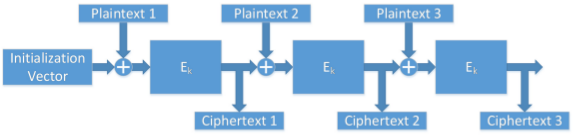
\includegraphics[width=0.7\textwidth]{figures/CBC.png}
\caption{CBC Ablauf}
\end{figure}

\begin{itemize}
    \item Initialization Vector
    \item Need not be secret
    \item Must be unpredictable
    \item Encryption cannot be performed in parallel
    \item Bit errors in a ciphertext block will affect decryption of the actual and the subsequent block
\end{itemize}

\hypertarget{decryption}{%
\subsubsection{Decryption}\label{decryption}}

\begin{figure}[H]
\centering
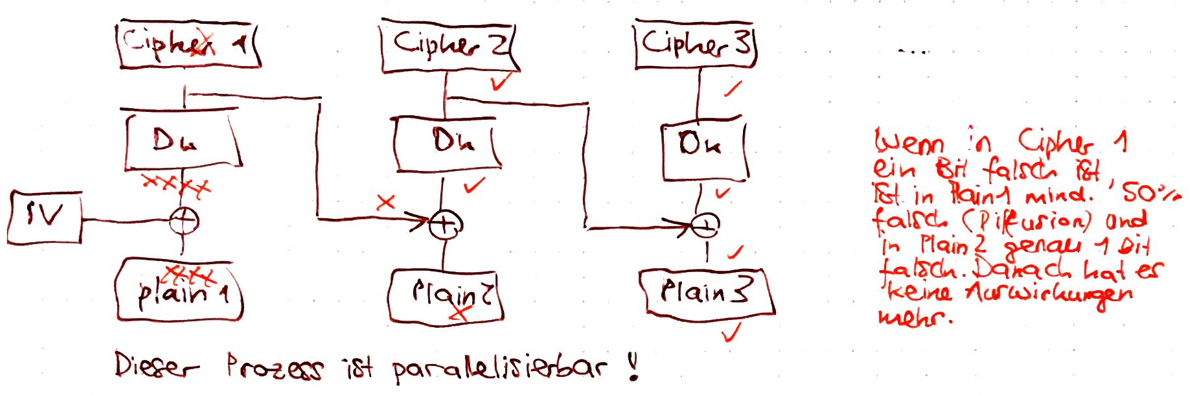
\includegraphics[width=0.8\textwidth]{figures/cfb_decryption.png}
\caption{CFB Decryption}
\end{figure}


\hypertarget{cipher-feedback---cfb}{%
\subsection{Cipher Feedback - CFB}\label{cipher-feedback---cfb}}

\begin{figure}[H]
\centering
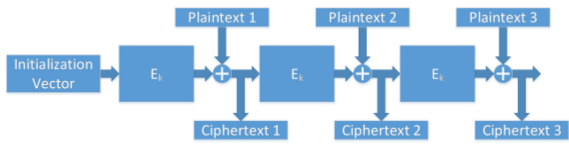
\includegraphics[width=0.7\textwidth]{figures/CFB.png}
\caption{CFB Ablauf}
\end{figure}

\begin{itemize}
    \item Feedback of ciphertext blocks into the input of the encryption algorithm
    \item Encryption cannot be performed in parallel
    \item Errors in a ciphertext block will affect decryption of actual and subsequent block (Big advantage!)
\end{itemize}


\hypertarget{output-feedback---ofb}{%
\subsection{Output Feedback - OFB}\label{output-feedback---ofb}}

\begin{figure}[H]
\centering
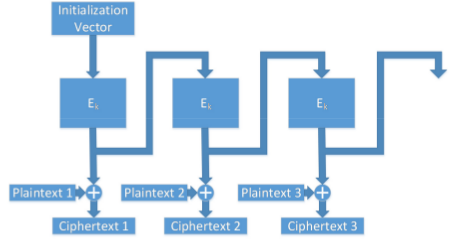
\includegraphics[width=0.7\textwidth]{figures/OFB.png}
\caption{OFB Ablauf}
\end{figure}

\begin{itemize}
    \item Encryption algorithm is used as a pseudo random generator → additive stream cipher
    \item IV must be unique for each execution of the mode (but not unpredictable)
    \item Needs synchronization between transmitter and receiver
    \item No error propagation
\end{itemize}

\hypertarget{counter---ctr}{%
\subsection{Counter - CTR}\label{counter---ctr}}

\begin{figure}[H]
\centering
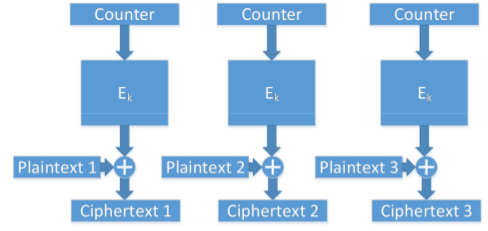
\includegraphics[width=0.7\textwidth]{figures/CTR.png}
\caption{CTR Ablauf}
\end{figure}

\begin{itemize}
    \item Encryption/Decryption can be performed in parallel
    \item Each counter value should only be used once with the same key → Nonce (Number used only once)
    \item No error propagation
\end{itemize}

\clearpage